\documentclass[10pt,twocolumn]{article}

\usepackage[pdftex]{graphicx}
\usepackage{caption}

\captionsetup{justification=centering}

\pagenumbering{arabic}
\setcounter{page}{201}

\hoffset=0in  
\voffset=-1in

\setlength{\columnwidth}{5in}
\setlength{\columnsep}{0.3in}
\setlength{\textheight}{9.5in}

\begin{document}
\small
{\setlength{\parindent}{0.3in} computing is carried out;}
\begin{itemize}
    \item To input video information, a camera 
(Video Camera Unit – VCU) is used designed to solve 
computer vision problems: detecting and tracking the user’s
face in the frame, identifying the user, recognizing
the emotions of the subject in the frame based on
frames from the video stream. According to the
general scheme of the system model 1, the camera
transmits the video stream to the computer vision
module (computer vision pipeline), and only then
the information is sent to the internal part of the
system for further processing. The peculiarity of
the proposed solution, which gives it additional
flexibility, is that the computer vision module can
be deployed both on the single-board computer itself
and on a separate machine (for example, a PC or
a specialized device designed to solve problems of
this type). Therefore, the camera can be connected
both to a single-board computer directly and to
an external device that will transmit information
through the abovementioned module to the central
device where the OSTIS system core is run. The
scheme of the hardware architecture considers the
option when the camera is connected directly;
    \item To speed up the performance of
operations on vectors and matrices when calculating neural networks
on hardware with limited resources, which include
single-board computers, it is proposed to use tensor
coprocessors (Tensor Processing Unit – TPU) for
neural network calculations.
\end{itemize}
Let us focus on each of the hardware components of
the system and consider them in more detail.

\setlength{\parskip}{-0.1cm}

\begin{flushleft}
\textit{A. Single-board computer}
\end{flushleft}

A single-board computer (SBC) is a computer set up
on a single printed circuit board, on which a microprocessor, RAM, I/O systems and other modules necessary for the operation of a computer are installed [22], [23].\\

As the basis of the hardware platform, it was proposed
to use a single-board computer, since such a form factor,
on the one hand, can provide the necessary and sufficient
runtime environment for the OSTIS Technology in terms
of performance and functionality and, on the other hand,
preserve the minimum weight-and-dimensional and cost
characteristics of computing tools, including for solving
problems connected with the Internet of things and the
usage of OSTIS within the framework of the “Edge
Computing and AI” [24], [25] concept.\\

We have reviewed and compared the models of singleboard computers on the local and international markets
that are available for delivery to the territory of the
Republic of Belarus. The model lines of computers from
such manufacturers as Interl NUX, LattePanda, Rock Pi,
UDOO, ODYSSEY [26] were considered. We have set
the maximum cost of a single-board computer, so that it\\

\begin{figure}[h]
  \setcounter{figure}{12}
  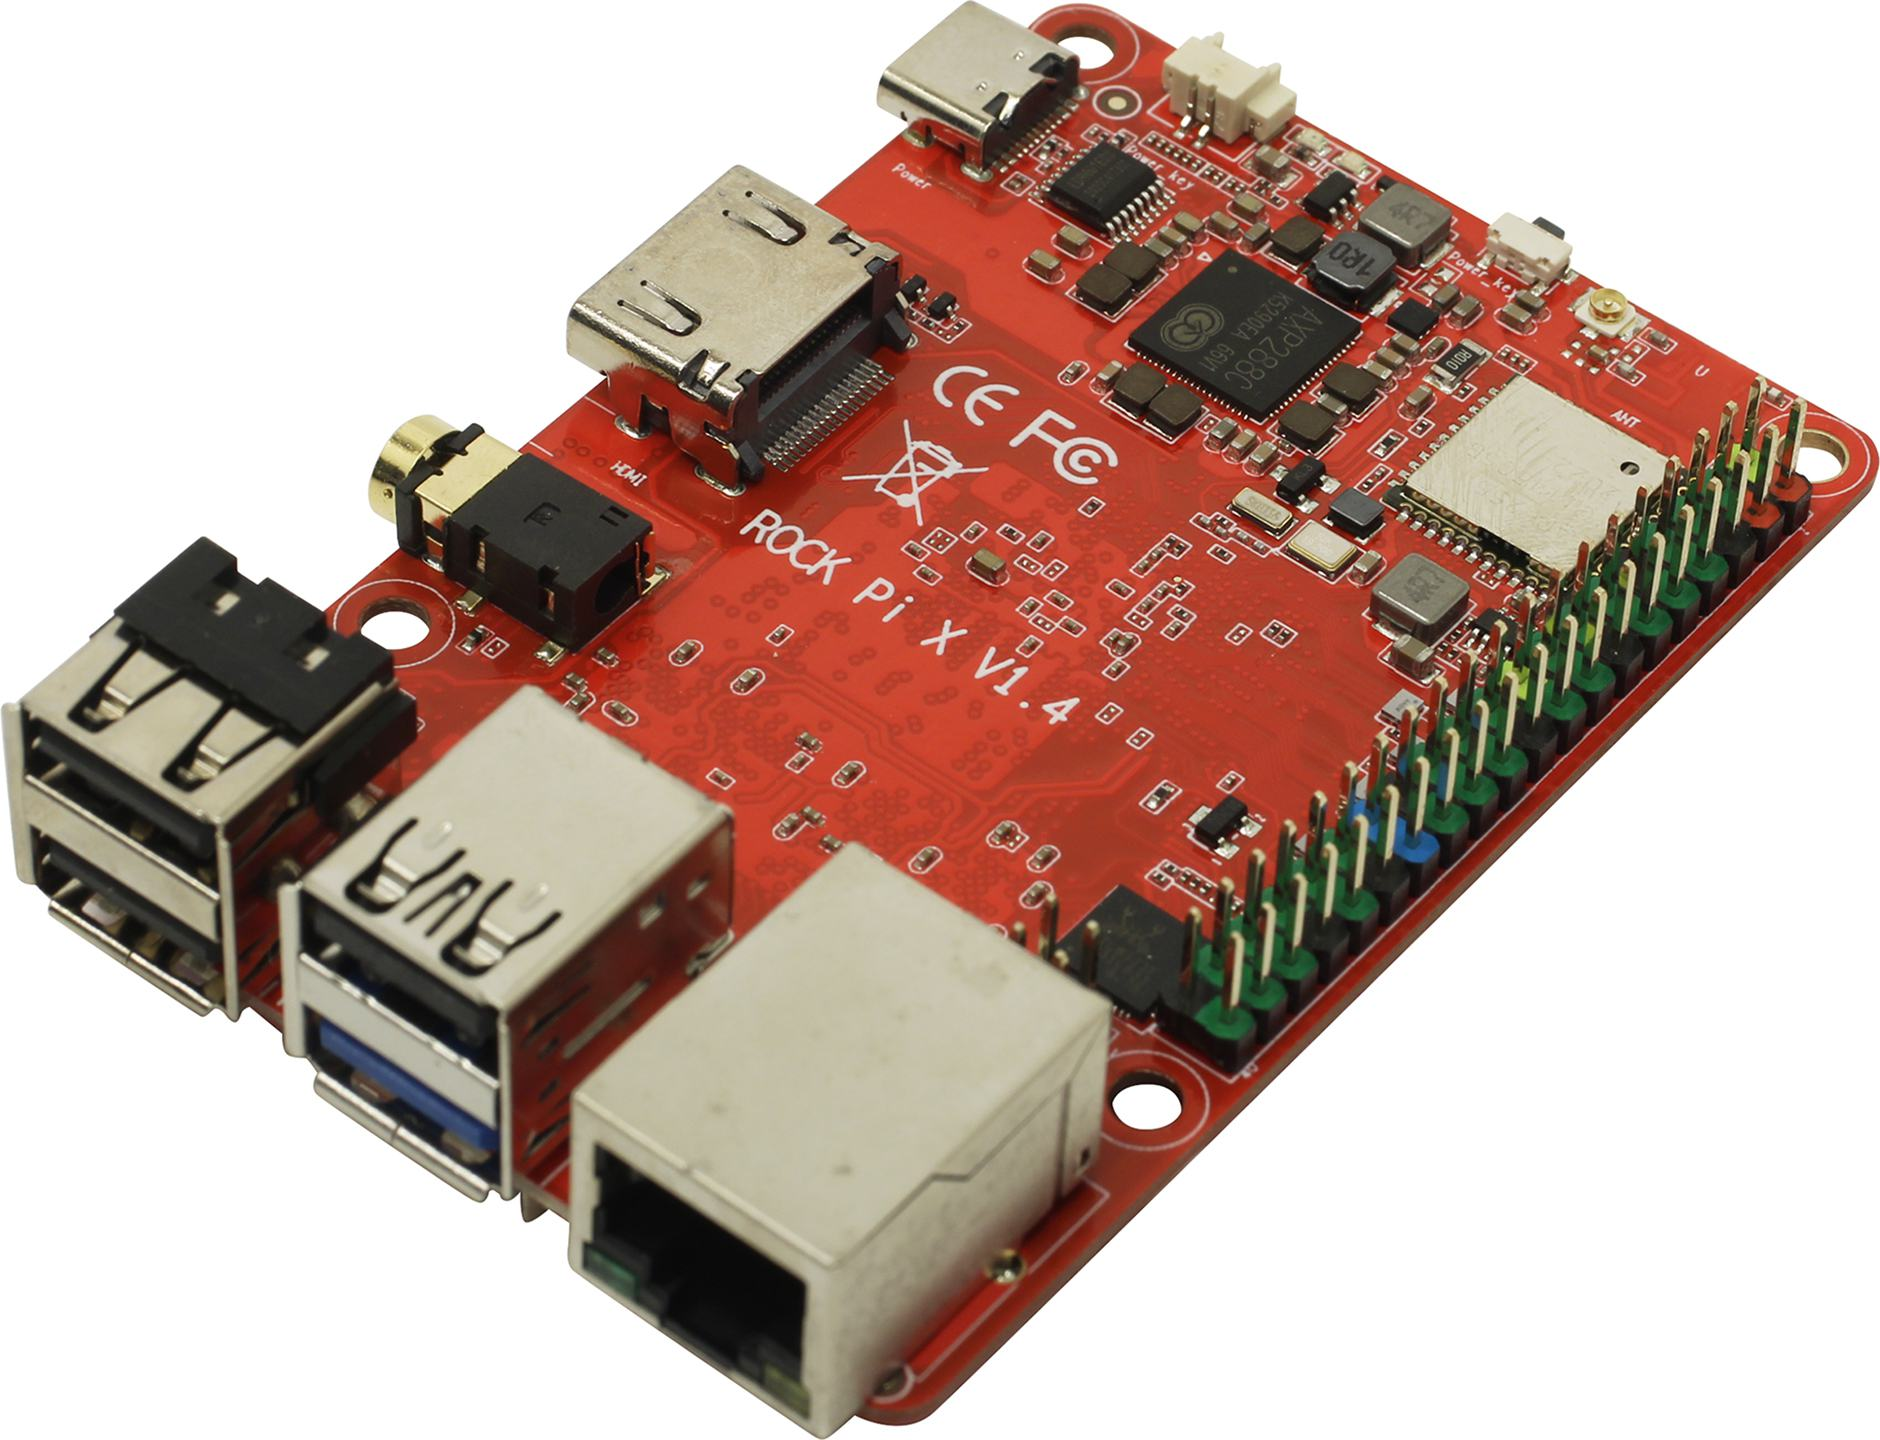
\includegraphics[width=\linewidth]{raspberry.jpg}
  \caption{A single-board computer “Rock PI X Model B”}
\end{figure}

\begin{figure}[h]
  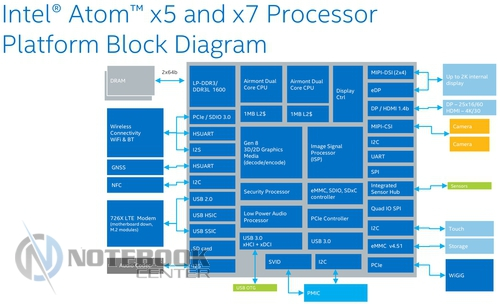
\includegraphics[width=\linewidth]{diagram.jpg}
  \caption{A single-board computer “Rock PI X Model B”}
\end{figure}

does not significantly exceed the cost of the option for
the ARM architecture. The set cost was no more than
\$100, which significantly narrowed the search area.\\

Among the currently available models of single-board
computers, the Rock Pi computer has become the most
preferred option, namely the Rock PI X Model B model
[27], the appearance of which is shown in fig. 13.\\

The functional diagram of the CPU [28], [29] is shown
in figure 14.\\

A distinctive feature of this single-board computer is
the presence of ROM based on eMMC, which allows
ensuring the functioning of the system and high-speed
access to data on a solid-state drive without using an
external SD drive. The maximum available capacity is
128 GB. The proposed architecture uses a version with
32 GB of memory, which is sufficient to contain the OS
as well as the necessary software modules and OSTIS
intelligent agents.\\

\textit{B. Video camera}\\

It is an element of the system, through which a video
stream is received and transmitted to a single-board
computer to solve subproblems connected with computer
vision and recognition of visual images. It acts as\\

\end{document}
